\chapter{Introduction}

See Chapter~\ref{chapter2}, read~\cite{goodfellow_generative_2014}.\\
The smooth boi can be seen on Fig.~\ref{subfig:smooth_boi}, and the outlined boi on Fig.~\ref{subfig:smooth_boi}. The whole figure is Fig.~\ref{fig:my_label}.

A derivative:
$$\diff{x}{y} = 2\pi x y$$
Insane!

And here we typeset COMET in smallcaps: \COMET. This \acrshort{COMET} is an \emph{acronym}. You can click it to see what it means.

\begin{figure}
    \centering
    \subfloat[A smooth boi]{
    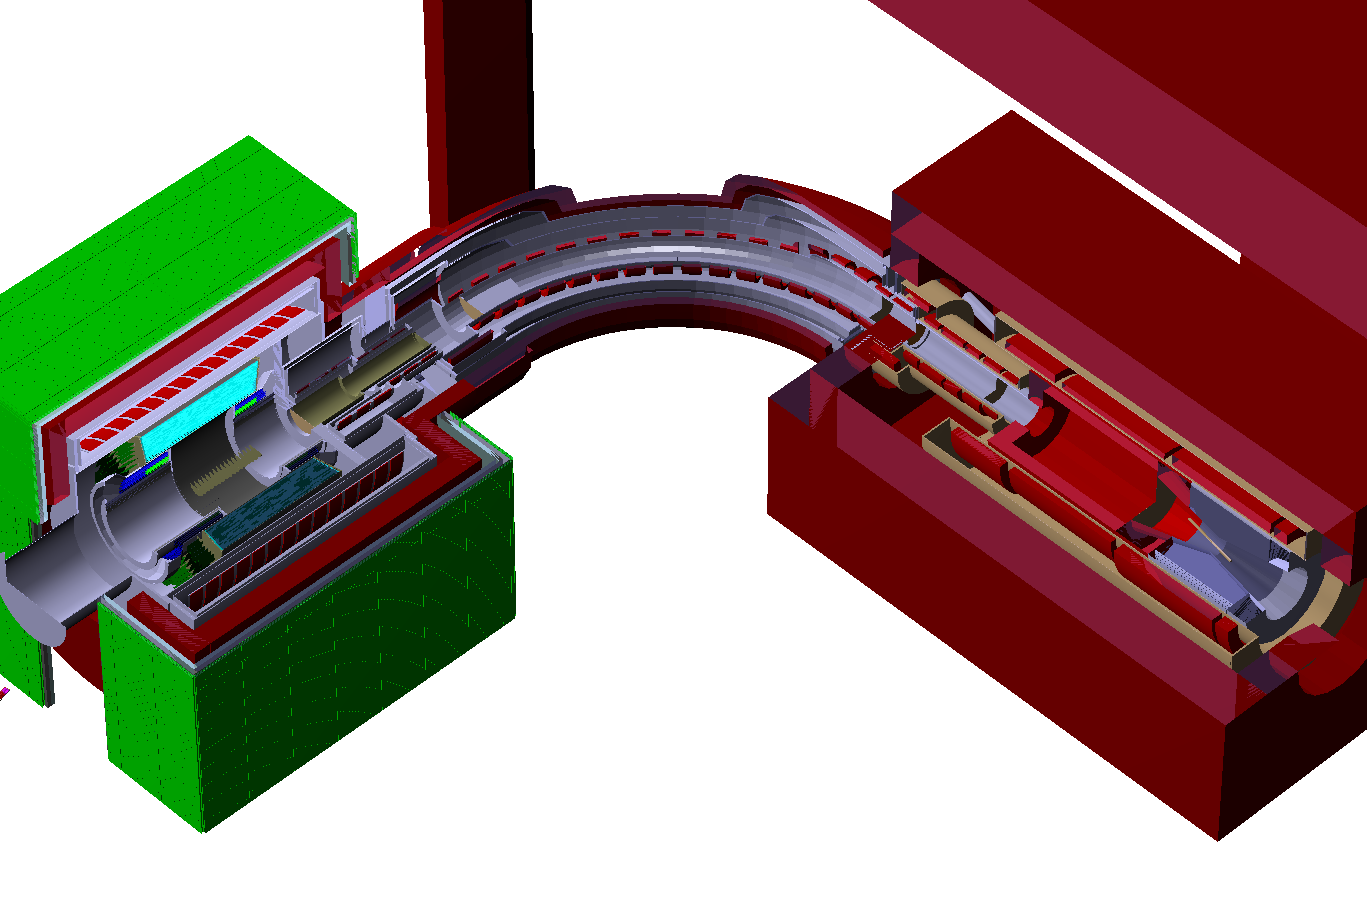
\includegraphics[width=0.5\textwidth]{viewer_smooth.png}
    \label{subfig:smooth_boi}
    }
    \subfloat[An outlined boi]{
    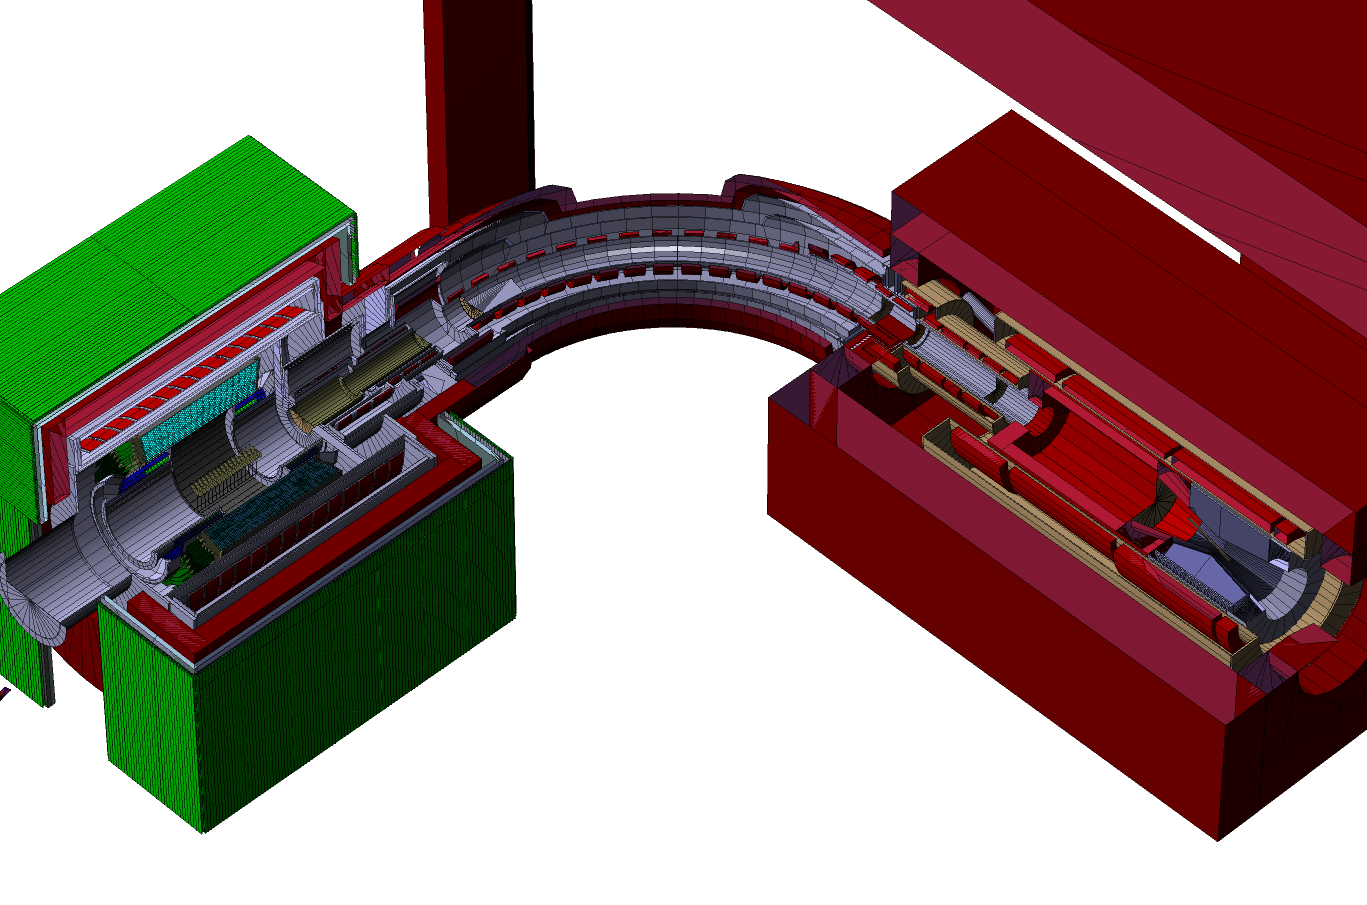
\includegraphics[width=0.5\textwidth]{viewer_outline2.png}
    \label{subfig:outlined_boi}
    }
    \caption{Phase-I cutaway geometries.}
    \label{fig:my_label}
\end{figure}

Here we cite the COMET TDR~\cite{the_comet_collaboration_comet_2020} and the upper limit on the branching ratio of $\mu^- + \textrm{Al} \rightarrow e^- + \textrm{Al}$, $7\times 10^{-13}$, by the SINDRUM-II experiment~\cite{Bertl:2006up}.
